\section{Merge Reduction}\seclabel{MergeReduction}
In \secref{InvariantClosure}, we discussed how \invariantconfluence{} is
fundamentally a property of reachability and that \invariantclosure{} is
sufficient but not necessary for \invariantconfluence{} because it fails to
incorporate any notion of reachability. Using this intuition, we established
\thmref{IclosureEquivalentIconfluence} and then exploited the theorem in
\algoref{InteractiveDecisionProcedure}. In this section, we again take
advantage of this intuition to develop a new sufficient condition for
\invariantconfluence{} that can be checked without user interaction and that
covers some cases not covered by \invariantclosure{}.

An expression $e = t_1(t_2(\ldots(t_n(s))\ldots))$ is \defword{merge-free} if
does not contain any merges (i.e.\ it is generated by the grammar $e ::= s \mid
t(e)$). An object $O = (S, \join)$ is \defword{merge-reducible} with respect to
a start state $s_0 \in S$, a set of transactions $T$, and an invariant $I$,
abbreviated \defword{\sTImergereducible}, if for every pair $e_1$ and $e_2$ of
merge-free \sTIreachable{} expressions, there exists some merge-free
\sTIreachable{} expression $e_3$ that evaluates to the same state as $e_1 \join
e_2$. Intuitively, if $O$ is merge-reducible, we can replace $e_1 \join e_2$
(which has one merge) with $e_3$ (which has no merges) to obtain an equivalent
expression with fewer merges.

\begin{example}\examplelabel{MergeReducible}
  Consider the distributed object $O = (\ints, \max)$ consisting of integers
  merged by the max function. Our start state state $s_0 = 0$ and our invariant
  $I = \setst{x \in \ints}{x \geq 0}$. Our set $T$ of transactions is the
  infinite set $T = \setst{t_y}{y \in \ints}$ where $t_y(x) = x + y$ is a
  transaction that adds $y$ to the state. For example, $t_2$ is a transaction
  that adds $2$ to the state, and $t_{-3}$ is a transaction which subtracts $3$
  from the state.
  %
  $O$ is \sTImergereducible{}. Consider two merge-free \sTIreachable{}
  expressions $e_1$ and $e_2$ that evaluate to states $x_1$ and $x_2$. Without
  loss of generality, assume $x_1 \geq x_2$. Then, we can replace $e_1 \join
  e_2$ (which evaluates to $x_1$) with $e_1$. We can also replace it with
  $t_{x_1}(0)$.
\end{example}

\begin{example}\examplelabel{NotMergeReducible}
  Consider the distributed object $O = (\set{X \subseteq \ints}, \join)$ in
  which each state is a set of integers and where $X_1 \join X_2 = \set{y}$
  where $y = \sum_{x \in X_1} x + \sum_{x \in X_2} x$. Our start state state
  $s_0 = \emptyset{}$ and our invariant $I = \setst{X}{\forall x \in X.\ x \
  \text{is even}}$. Our set $T$ of transactions is the set $T = \set{t_0, t_2,
  t_4}$ where $t_i(X) = X \cup \set{i}$ is a transaction that adds $i$ to the
  state. For example, $t_2(\set{0}) = \set{0, 2}$.
  %
  $O$ is \emph{not} \sTImergereducible{}. Consider the two merge-free
  \sTIreachable{} expressions $e_1 = t_2(\emptyset)$ and $e_2 =
  t_4(\emptyset)$. $e_1 \join e_2$ evaluates to $\set{6}$, but there does not
  exist a merge-free expression that evaluates to $\set{6}$.
\end{example}

{\begin{figure*}[ht]
  \centering

  \tikzstyle{s0color}=[fill=flatred]
  \tikzstyle{s1color}=[fill=flatgreen]
  \tikzstyle{s2color}=[fill=flatdenim]
  \tikzstyle{s3color}=[fill=flatorange]
  \tikzstyle{s4color}=[fill=flatyellow]
  \tikzstyle{s5color}=[fill=flatcyan]
  \tikzstyle{s6color}=[fill=flatpurple]
  \tikzstyle{s7color}=[fill=flatblue]
  \tikzstyle{astedge}=[thick]
  \tikzstyle{phantomstate}=[%
    shape=circle, inner sep=2pt, draw=white, line width=1pt, fill=white]
  \tikzstyle{state}=[%
    shape=circle, inner sep=2pt, draw=black, line width=1pt, text opacity=1,
    fill opacity=0.6]
  \newcommand{\internaltext}[1]{$\boldsymbol #1$}

  \begin{tikzpicture}[xscale=1.1]
    \begin{scope}[]
                         \node[state, s7color, label={[label distance=-0.1cm] 90:$s_7$}] (s7) at (0, 0) {\internaltext{\join}};
      \draw (s7)++(210:1) node[state, s3color, label={[label distance=-0.1cm] 90:$s_3$}] (s3)           {\internaltext{\join}};
      \draw (s7)++(-30:1) node[state, s6color, label={[label distance=-0.1cm] 90:$s_6$}] (s6)           {\internaltext{\join}};
      \draw (s3)++(240:1) node[state, s1color, label={[label distance=-0.2cm] 120:$s_1$}](s1)           {\internaltext{t}};
      \draw (s3)++(-60:1) node[state, s2color, label={[label distance=-0.2cm] 60:$s_2$}] (s2)           {\internaltext{u}};
      \draw (s6)++(240:1) node[state, s4color, label={[label distance=-0.2cm] 240:$s_4$}](s4)           {\internaltext{v}};
      \draw (s6)++(-60:1) node[state, s5color, label={[label distance=-0.2cm] 60:$s_5$}] (s5)           {\internaltext{w}};
      \draw (s1)++(-90:1) node[state, s0color]                                           (n1)           {\internaltext{s_0}};
      \draw (s2)++(-90:1) node[state, s0color]                                           (n2)           {\internaltext{s_0}};
      \draw (s4)++(-90:1) node[state, s0color]                                           (n4)           {\internaltext{s_0}};
      \draw (s5)++(-90:1) node[state, s0color]                                           (n5)           {\internaltext{s_0}};
      \draw[astedge] (s7) to (s3) to (s1) to (n1);
      \draw[astedge] (s7) to (s3) to (s2) to (n2);
      \draw[astedge] (s7) to (s6) to (s4) to (n4);
      \draw[astedge] (s7) to (s6) to (s5) to (n5);
      \coordinate (A) at (s5);
    \end{scope}
    \begin{scope}[xshift=125]
      \node[state, s7color, label={[label distance=-0.1cm] 90:$s_7$}] (s7) at (0, 0) {\internaltext{\join}};
      \draw (s7)++(210:1) node[state, s3color, label={[label distance=-0.1cm] 90:$s_3$}] (s3)           {\internaltext{p}};
      \draw (s7)++(-30:1) node[state, s6color, label={[label distance=-0.1cm] 90:$s_6$}] (s6)           {\internaltext{\join}};
      \draw (s6)++(240:1) node[state, s4color, label={[label distance=-0.2cm] 240:$s_4$}](s4)           {\internaltext{v}};
      \draw (s6)++(-60:1) node[state, s5color, label={[label distance=-0.2cm] 60:$s_5$}] (s5)           {\internaltext{w}};
      \draw (s3)++(-90:1) node[state, s0color]                                           (n3)           {\internaltext{s_0}};
      \draw (s4)++(-90:1) node[state, s0color]                                           (n4)           {\internaltext{s_0}};
      \draw (s5)++(-90:1) node[state, s0color]                                           (n5)           {\internaltext{s_0}};
      \draw[astedge] (s7) to (s3) to (n3);
      \draw[astedge] (s7) to (s6) to (s4) to (n4);
      \draw[astedge] (s7) to (s6) to (s5) to (n5);
    \end{scope}
    \begin{scope}[xshift=250]
      \node[state, s7color, label={[label distance=-0.1cm] 90:$s_7$}] (s7) at (0, 0) {\internaltext{\join}};
      \draw (s7)++(210:1) node[state, s3color, label={[label distance=-0.1cm] 90:$s_3$}] (s3)           {\internaltext{p}};
      \draw (s7)++(-30:1) node[state, s6color, label={[label distance=-0.1cm] 90:$s_6$}] (s6)           {\internaltext{q}};
      \draw (s3)++(-90:1) node[state, s0color]                                           (n3)           {\internaltext{s_0}};
      \draw (s6)++(-90:1) node[state, s0color]                                           (n6)           {\internaltext{s_0}};
      \draw[astedge] (s7) to (s3) to (n3);
      \draw[astedge] (s7) to (s6) to (n6);
    \end{scope}
    \begin{scope}[xshift=350]
                         \node[state, s7color, label={[label distance=-0.1cm] 90:$s_7$}] (s7) at (0, 0) {\internaltext{r}};
      \draw (s7)++(-90:1) node[state, s0color]                                           (n7)           {\internaltext{s_0}};
      \draw[astedge] (s7) to (n7);
    \end{scope}

    \draw[-latex, line width=3pt] (A) ++ (0.55, 0) to ++(1, 0);
    \draw[-latex, line width=3pt] (A) ++ (5, 0) to ++(1, 0);
    \draw[-latex, line width=3pt] (A) ++ (9, 0) to ++(1, 0);
  \end{tikzpicture}

  \caption{%
    An illustration of the proof of \thmref{ReducibilityImpliesIconfluence}. We
    begin with a reachable expression and convert it into a merge-free
    reachable expression by repeatedly replacing the merge of two merge-free
    reachable subexpressions with an equivalent merge-free reachable
    expression. In this example, we first replace $t(s_0) \join u(s_0)$ with
    $p(s_0)$. We then replace $v(s_0) \join w(s_0)$ with $q(s_0)$. Finally, we
    replace $p(s_0) \join q(s_0)$ with $r(s_0)$.
  }\figlabel{MergingDiagram}
\end{figure*}
}

\begin{theorem}\thmlabel{ReducibilityImpliesIconfluence}
  Given an object $O = (S, \join)$, a start state $s_0 \in S$, a set of
  transactions $T$, and an invariant $I$, if $I(s_0)$ and if $O$ is
  \sTImergereducible{}, then $O$ is \sTIconfluent{}.
\end{theorem}

\begin{proof}
  Intuitively, the proof of \thmref{ReducibilityImpliesIconfluence} is a
  straightforward induction. We begin with an \sTIreachable{} expression $e$
  and repeatedly replace any subexpression that merges two merge-free
  subexpressions with an equivalent merge-free reachable subexpression (which
  we can do because $O$ is merge-reducible). We repeat this process until $e$
  has been completely replaced with an equivalent merge-free reachable
  expression $e'$. Because $I(s_0)$ and because our system model only executes
  transactions that preserve the invariant, $e'$ (and hence $e$) is guaranteed
  to satisfy the invariant. Thus, all reachable states satisfy the invariant,
  so $O$ is \invariantconfluent{}. An illustration of this idea is given in
  \figref{MergingDiagram}.

  More formally, we prove by structural induction on $e$, that for all
  \sTIreachable{} expressions $e$, there exists a merge-free \sTIreachable{}
  expression $e'$ such that $eval(e) = eval(e')$.
  \begin{itemize}
    \item \textbf{Case 1: $e = s_0$.}
      Trivially, $e' = s_0$.

    \item \textbf{Case 2: $e = t(e_1)$.}
      $e_1$ is \sTIreachable{}, so by the inductive hypothesis, there exists a
      merge-free \sTIreachable{} expression $e_1'$ such that $eval(e_1) =
      eval(e_1')$. $t(e_1)$ is \sTIreachable{}, so $I(t(e_1))$. Because
      $eval(e_1) = eval(e_1')$, we know also that $I(t(e_1'))$. Thus, $t(e_1')$
      is \sTIreachable{} (and join free), so we can let $e' = t(e_1')$.

    \item \textbf{Case 3: $e = e_1 \join e_2$.}
      $e_1$ and $e_2$ are \sTIreachable{}, so by the inductive hypothesis,
      there exists equivalent merge-free \sTIreachable{} expressions $e_1'$ and
      $e_2'$. $O$ is \sTImergereducible{}, so there exists an equivalent
      merge-free \sTIreachable{} expression $e'$.
  \end{itemize}

  Consider an arbitrary \sTIreachable{} expression $e$ and it's equivalent
  merge-free \sTIreachable{} counterpart $e'$. $e'$ is either $s_0$ or
  $t(e'')$.  In either case, it satisfies the invariant, so $O$ is
  \sTIconfluent{}.
\end{proof}

Note that while merge-reducibility is a sufficient condition for
\invariantconfluence{}, it is not necessary. The object in
\exampleref{NotMergeReducible} is \invariantconfluent{} but not
merge-reducible.

Merge-reducibility is a sufficient condition for \invariantconfluence{}, but
unlike with \invariantclosure{}, it is not straightforward to automatically
determine if an object is merge-reducible. In \thmref{LatticeProperty}, we
outline a sufficient condition for merge-reducibility that is straightforward
to determine automatically.

\begin{theorem}\thmlabel{LatticeProperty}
  Given an object $O = (S, \join)$, a start state $s_0 \in S$, a set of
  transactions $T$, and an invariant $I$, if the following criteria are met,
  then $O$ is \sTImergereducible{} (and therefore \sTIconfluent{}).
  \begin{enumerate}
    \item
      $O$ is a join-semilattice. That is, $\join$ is associative ($(x \join y)
      \join z = x \join (y \join z)$), commutative ($x \join y = y \join x$),
      and idempotent ($x \join x = x$).

    \item
      For every $t \in T$, there exists some $s_t \in S$ such that for all $s
      \in S$, $t(s) = s \join s_t$. That is, every transaction $t$ is of the
      form $t(s) = s \join s_t$ for some constant $s_t$.

    \item
      For every pair of transactions $t_1, t_2 \in T$ and for all states $s \in
      S$, if $I(s)$, $I(t_1(s))$, and $I(t_2(s))$, then $I(t_1(s) \join
      t_2(s))$.

    \item
      $I(s_0)$.
  \end{enumerate}
\end{theorem}

\newcommand{\bart}[1]{\overline{t_{#1}}}
\newcommand{\baru}[1]{\overline{u_{#1}}}
\newcommand{\bartu}[2]{\bart{#1}(\baru{#2}(s_0))}
\begin{proof}
  Let
  \[
    \hfill
    e_1 = t_n(t_{n-1}(\ldots (t_1(s_0))\ldots))
    \hfill
  \]
  and
  \[
    \hfill
    e_2 = u_m(u_{m-1}(\ldots (u_1(s_0))\ldots))
    \hfill
  \]
  be two arbitrary merge-free \sTIreachable{} expressions.
  For ease of notation, let
  \[
    \hfill
    \bart{i} = t_i(\ldots(t_1(s_0))\ldots)
    \quad\text{and}\quad
    \baru{j} = u_j(\ldots(u_1(s_0))\ldots)
    \hfill
  \]
  We want to show that there exists some merge-free \sTIreachable{} expression
  that is equivalent to $e_1 \join e_2$.
  %
  To do so, we prove by strong induction on $k \in \nats$ that if $k = i + j$
  where $0 \leq i \leq n$ and $0 \leq j \leq m$, $\bartu{i}{j}$ is
  \sTIreachable{} and $eval(\bartu{i}{j}) = eval(\bart{i}(s_0) \join
  \baru{j}(s_0))$.
  \begin{itemize}
    \item \textbf{Case $k = 0$.}
      $i = j = 0$, so $\bartu{0}{0} = s_0$ which is trivially \sTIreachable{}
      and equivalent to $\bart{0}(s_0) \join \baru{0}(s_0) = s_0 \join s_0$
      which evaluates to $s_0$ (because $\join$ is idempotent).

    \item \textbf{Case $k = 1$.}
      Without loss of generality, assume $i = 1$ and $j = 0$. Then,
      $
        \bartu{1}{0} = t_1(s_0)
      $ which is \sTIreachable{} because it is a subexpression of $\bart{n}$
      which is \sTIreachable{}. Moreover, it is equivalent to $\bart{1}(s_0)
      \join \baru{0}(s_0) = t_1(s_0) \join s_0$ which evaluates to $s_{t_1}
      \join s_0 \join s_0 = s_{t_1} \join s_0 = t_1(s_0)$ for some $s_{t_1} \in
      S$.

    \item \textbf{Case $k \geq 2$.}
      If $i = 0$, then $j = k$ and $\baru{k}(s_0)$ is \sTIreachable{} because
      it is a subexpression of $\baru{m}(s_0)$. Also, it is equivalent to
      $\bart{0}(s_0) \join \baru{k}(s_0)$ which evaluates to $\baru{k}(s_0)$.
      %
      The symmetric result holds if $j = 0$.

      Otherwise, $i, j > 1$. Let
      \begin{align*}
        e_{i-1,j-1} &= \bartu{i-1}{j-1} \\
        e_{i,j-1} &= \bartu{i}{j-1} \\
        e_{i-1,j} &= \bartu{i-1}{j}
      \end{align*}
      By the inductive hypothesis, $e_{i-1,j-1}$, $e_{i,j-1}$, and $e_{i-1,j}$
      are all \sTIreachable{}. By condition 3 (with $s = eval(e_{i-1,j-1})$,
      $t_1$ = $t_i$, and $t_2 = u_j$), $I(e_{i,j-1} \join e_{i-1,j})$.
      $e_{i,j-1} \join e_{i-1,j} = t_i(e_{i-1,j}) = u_j(e_{i,j-1}) =
      \bartu{i}{j}$, so $I(\bartu{i}{j})$. Therefore, $\bartu{i}{j}$ is
      \sTIreachable{}.
  \end{itemize}
\end{proof}

{% Implication.
\tikzstyle{impl}=[-implies, double distance=3pt]

% Transaction.
\tikzstyle{txn}=[thick, -latex]

% Dashed transaction.
\tikzstyle{dtxn}=[thick, -latex, dashed]

% G transaction.
\tikzstyle{gtxn}=[thick, -latex, decorate, decoration={zigzag}]

% Dashed G transaction.
\tikzstyle{dgtxn}=[thick, -latex, densely dashed, decorate, decoration={zigzag}]

% Invariant node.
\newcommand{\inode}[3][]{
  \node[draw, shape=circle, minimum width=0.4cm] (#2) at (#3) {};
  \node[fill, shape=circle, #1] () at (#3) {};
}

% Normal node.
\newcommand{\nnode}[3][]{
  \node[fill, shape=circle, #1] (#2) at (#3) {};
}

\newcommand{\baseedges}{
  \begin{scope}[on background layer]
    \draw[txn] (03) -- (13) node[midway, above]{$u_1$};
    \draw[txn] (13) -- (23) node[midway, above]{$u_2$};
    \draw[txn] (23) -- (33) node[midway, above]{$u_3$};
    \draw[txn] (03) -- (02) node[midway, left]{$t_1$};
    \draw[txn] (02) -- (01) node[midway, left]{$t_2$};
    \draw[txn] (01) -- (00) node[midway, left]{$t_3$};
    \draw[dtxn] (00) -- (30);
    \draw[dtxn] (33) -- (30);
  \end{scope}
}

\begin{figure*}[ht]
  \centering
  \newcommand{\onescale}{1}

  \begin{subfigure}[b]{0.24\textwidth}
    \centering
    \begin{tikzpicture}[scale=\onescale]
      \foreach \x/\y in {
             1/3, 2/3, 3/3,
        0/2,
        0/1,
        0/0%
      } {
        \inode{\x\y}{\x, \y}
      }
      \foreach \x/\y in {0/3} {
        \inode[flatred]{\x\y}{\x, \y}
      }
      \nnode{30}{3, 0}
      \baseedges{}
    \end{tikzpicture}
    \caption{$k=0$}
    \label{fig:one-is-enough-base}
  \end{subfigure}
  \begin{subfigure}[b]{0.24\textwidth}
    \centering
    \begin{tikzpicture}[scale=\onescale]
      \foreach \x/\y in {
        0/3,      2/3, 3/3,
        %
        0/1,
        0/0%
      } {
        \inode{\x\y}{\x, \y}
      }
      \foreach \x/\y in {0/2, 1/3} {
        \inode[flatred]{\x\y}{\x, \y}
      }
      \nnode{30}{3, 0}
      \baseedges{}
    \end{tikzpicture}
    \caption{$k=1$}
    \label{}
  \end{subfigure}%
  \begin{subfigure}[b]{0.24\textwidth}
    \centering
    \begin{tikzpicture}[scale=\onescale]
      \foreach \x/\y in {
        0/3, 1/3,      3/3,
        0/2,
        %
        0/0%
      } {
        \inode{\x\y}{\x, \y}
      }
      \foreach \x/\y in {0/1, 1/2, 2/3} {
        \inode[flatred]{\x\y}{\x, \y}
      }
      \nnode{30}{3, 0}
      \baseedges{}
      \draw[txn] (02) -- (12) node[midway, above] {$u_1$};
      \draw[txn] (13) -- (12) node[midway, left]  {$t_1$};
    \end{tikzpicture}
    \caption{$k=2$}
    \label{}
  \end{subfigure}%
  \begin{subfigure}[b]{0.24\textwidth}
    \centering
    \begin{tikzpicture}[scale=\onescale]
      \foreach \x/\y in {
        0/3, 1/3, 2/3,
        0/2, 1/2,
        0/1%
        %
      } {
        \inode{\x\y}{\x, \y}
      }
      \foreach \x/\y in {0/0, 1/1, 2/2, 3/3} {
        \inode[flatred]{\x\y}{\x, \y}
      }
      \nnode{30}{3, 0}
      \baseedges{}
      \draw[txn] (02) -- (12) node[midway, above] {$u_1$};
      \draw[txn] (13) -- (12) node[midway, left]  {$t_1$};
      \draw[txn] (01) -- (11) node[midway, above] {$u_1$};
      \draw[txn] (12) -- (11) node[midway, left]  {$t_2$};
      \draw[txn] (12) -- (22) node[midway, above] {$u_2$};
      \draw[txn] (23) -- (22) node[midway, left]  {$t_1$};
    \end{tikzpicture}
    \caption{$k=3$}
    \label{}
  \end{subfigure}

  \begin{subfigure}[b]{0.3\textwidth}
    \centering
    \begin{tikzpicture}[scale=\onescale]
      \foreach \x/\y in {
        0/3, 1/3, 2/3, 3/3,
        0/2, 1/2, 2/2,
        0/1, 1/1,
        0/0%
      } {
        \inode{\x\y}{\x, \y}
      }
      \foreach \x/\y in {1/0, 2/1, 3/2} {
        \inode[flatred]{\x\y}{\x, \y}
      }
      \nnode{30}{3, 0}
      \baseedges{}
      \draw[txn] (02) -- (12) node[midway, above] {$u_1$};
      \draw[txn] (13) -- (12) node[midway, left]  {$t_1$};
      \draw[txn] (01) -- (11) node[midway, above] {$u_1$};
      \draw[txn] (12) -- (11) node[midway, left]  {$t_2$};
      \draw[txn] (12) -- (22) node[midway, above] {$u_2$};
      \draw[txn] (23) -- (22) node[midway, left]  {$t_1$};
      \draw[txn] (00) -- (10) node[midway, above] {$u_1$};
      \draw[txn] (11) -- (10) node[midway, left]  {$t_3$};
      \draw[txn] (11) -- (21) node[midway, above] {$u_2$};
      \draw[txn] (22) -- (21) node[midway, left]  {$t_2$};
      \draw[txn] (22) -- (32) node[midway, above] {$u_3$};
      \draw[txn] (33) -- (32) node[midway, left]  {$t_1$};
    \end{tikzpicture}
    \caption{$k=4$}
    \label{}
  \end{subfigure}%
  \begin{subfigure}[b]{0.3\textwidth}
    \centering
    \begin{tikzpicture}[scale=\onescale]
      \foreach \x/\y in {
        0/3, 1/3, 2/3, 3/3,
        0/2, 1/2, 2/2, 3/2,
        0/1, 1/1, 2/1,
        0/0, 1/0%
      } {
        \inode{\x\y}{\x, \y}
      }
      \foreach \x/\y in {2/0, 3/1} {
        \inode[flatred]{\x\y}{\x, \y}
      }
      \nnode{30}{3, 0}
      \baseedges{}
      \draw[txn] (02) -- (12) node[midway, above] {$u_1$};
      \draw[txn] (13) -- (12) node[midway, left]  {$t_1$};
      \draw[txn] (01) -- (11) node[midway, above] {$u_1$};
      \draw[txn] (12) -- (11) node[midway, left]  {$t_2$};
      \draw[txn] (12) -- (22) node[midway, above] {$u_2$};
      \draw[txn] (23) -- (22) node[midway, left]  {$t_1$};
      \draw[txn] (00) -- (10) node[midway, above] {$u_1$};
      \draw[txn] (11) -- (10) node[midway, left]  {$t_3$};
      \draw[txn] (11) -- (21) node[midway, above] {$u_2$};
      \draw[txn] (22) -- (21) node[midway, left]  {$t_2$};
      \draw[txn] (22) -- (32) node[midway, above] {$u_3$};
      \draw[txn] (33) -- (32) node[midway, left]  {$t_1$};
      \draw[txn] (10) -- (20) node[midway, above] {$u_2$};
      \draw[txn] (21) -- (20) node[midway, left]  {$t_3$};
      \draw[txn] (21) -- (31) node[midway, above] {$u_3$};
      \draw[txn] (32) -- (31) node[midway, left]  {$t_2$};
    \end{tikzpicture}
    \caption{$k=5$}
    \label{}
  \end{subfigure}%
  \begin{subfigure}[b]{0.3\textwidth}
    \centering
    \begin{tikzpicture}[scale=\onescale]
      \foreach \x/\y in {
        0/3, 1/3, 2/3, 3/3,
        0/2, 1/2, 2/2, 3/2,
        0/1, 1/1, 2/1, 3/1,
        0/0, 1/0, 2/0%
      } {
        \inode{\x\y}{\x, \y}
      }
      \inode[flatred]{30}{3, 0}
      \baseedges{}
      \draw[txn] (02) -- (12) node[midway, above] {$u_1$};
      \draw[txn] (13) -- (12) node[midway, left]  {$t_1$};
      \draw[txn] (01) -- (11) node[midway, above] {$u_1$};
      \draw[txn] (12) -- (11) node[midway, left]  {$t_2$};
      \draw[txn] (12) -- (22) node[midway, above] {$u_2$};
      \draw[txn] (23) -- (22) node[midway, left]  {$t_1$};
      \draw[txn] (00) -- (10) node[midway, above] {$u_1$};
      \draw[txn] (11) -- (10) node[midway, left]  {$t_3$};
      \draw[txn] (11) -- (21) node[midway, above] {$u_2$};
      \draw[txn] (22) -- (21) node[midway, left]  {$t_2$};
      \draw[txn] (22) -- (32) node[midway, above] {$u_3$};
      \draw[txn] (33) -- (32) node[midway, left]  {$t_1$};
      \draw[txn] (10) -- (20) node[midway, above] {$u_2$};
      \draw[txn] (21) -- (20) node[midway, left]  {$t_3$};
      \draw[txn] (21) -- (31) node[midway, above] {$u_3$};
      \draw[txn] (32) -- (31) node[midway, left]  {$t_2$};
      \draw[txn] (20) -- (30) node[midway, above] {$u_3$};
      \draw[txn] (31) -- (30) node[midway, left]  {$t_3$};
    \end{tikzpicture}
    \caption{$k=6$}
    \label{}
  \end{subfigure}

  \caption{Illustration of the proof of \thmref{LatticeProperty} for $n=m=3$}
  \figlabel{DiamondProofDiagram}
\end{figure*}
}

An illustration of this proof is given in \figref{DiamondProofDiagram}. We
arrange the expressions $e_1$ and $e_2$ as the left and top edges of a square
grid. Each point in the grid represents a state (with $s_0$ in the top left
corner), and each edge represents the application of a transaction. A state is
circled if we know it satisfies the invariant.
%
Condition (1) and (2) tell us that the order in which we apply transactions is
immaterial. Thus, if we begin at the top left of the square and walk to any
other point in the square, applying transactions along the way, it does not
matter which path we take. They are all equivalent. Condition (4) tells us that
the top-left corner satisfies the invariant. We induct to repeatedly apply
condition (3) to ``fill in'' the square, one block at a time. In iteration $k$,
we discover that all points with a Manhattan distance of $k$ from the top left
corner satisfy the invariant. Ultimately, we conclude that the bottom right
corner (i.e., $e_1 \join e_2$) satisfies the invariant and is equivalent to
$\bartu{n}{m}$.

\thmref{IclosureImpliesIconfluence} states that \invariantclosure{} is a
sufficient condition for \invariantconfluence{}, and \thmref{LatticeProperty}
states that criteria (1) -- (4) are sufficient conditions for
\invariantconfluence{}. How do these sufficient conditions relate to one
another?  Clearly, not all \invariantclosed{} objects are semilattices, so
\invariantclosure{} does not imply criteria (1) -- (4). Conversely, there are
some objects that satisfy criteria (1) -- (4) that are not
\invariantclosed{}. Here's one example.

\begin{example}\examplelabel{TwoSets}
  Let $O = (\mathcal{P}(\nats), \cup)$ where $\mathcal{P}(\nats)$ is the power
  set of the natural numbers. Our start state $s_0 = \set{0}$ is the set of
  $0$. Let $t_Y(X) = X \cup Y$ be the transaction that unions $Y$ with its
  argument $X$. Our set $T = \setst{t_Y}{Y \subseteq \nats}$ of transactions
  consists of all possible $t_Y$. Our invariant $I$ consists of all non-empty
  sets $X$ that contain only even or only odd elements. That is, $I = \setst{X
  \subseteq 2\nats}{X \neq \emptyset} \cup \setst{X \subseteq 2\nats + 1}{X
  \neq \emptyset}$.

  Criteria (1), (2), (3) and (4) are all satisfied. However, $O$ is not
  \Iclosed{}. Let $s_1 = \set{0}$ and $s_2 = \set{1}$. Then, $I(s_1)$ and
  $I(s_2)$, but letting $s_3 = s_1 \cup s_2 = \set{0, 1}$, $\lnot I(s_3)$.

  Here's why criterion (3) is satisfied. If $s$ is an arbitrary state that
  satisfies $I$, then it is non-empty and contains, without loss of generality,
  only even integers. If $t_1$ and $t_2$ are arbitrary transactions such that
  $I(t_1(s))$ and $I(t_2(s))$, then $t_1(s)$ and $t_2(s)$ are also non-empty
  and contain only even integers. Thus, $t_1(s) \cup t_2(s)$ is clearly
  non-empty and contains only even integers, so $I(t_1(s) \join t_2(s))$.
\end{example}

{\begin{figure}[t]
  \centering
  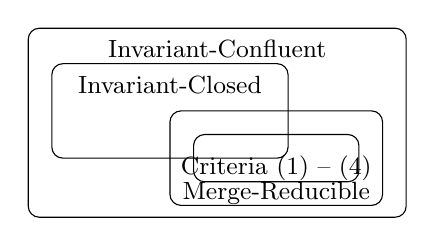
\begin{tikzpicture}[scale=0.3]
    \draw[rounded corners] (0, 0) rectangle (16, 8);
    \draw[rounded corners] (1, 2.5) rectangle (11, 6.5);
    \draw[rounded corners] (6, 0.5) rectangle (15, 4.5);
    \draw[rounded corners] (7, 1.5) rectangle ++(7, 2);
    \node[inner sep=0pt, anchor=north] at (8, 7.5) {\small Invariant-Confluent};
    \node[inner sep=0pt, anchor=north] at (6, 6) {\small Invariant-Closed};
    \node[inner sep=0pt, anchor=south] at (10.5, 1.5) {\small Criteria (1) -- (4)};
    \node[inner sep=0pt, anchor=south] at (10.5, 0.5) {\small Merge-Reducible};
  \end{tikzpicture}
  \caption{%
    The relationship between invariant-closure, merge-reducibility, criteria
    (1) -- (4) from \thmref{LatticeProperty}, and invariant-confluence.
  }\figlabel{IclosureVsReducible}
\end{figure}
}

\Invariantclosure{} is not necessary for \invariantconfluence{} because it
fails to incorporate any notion of reachability. Criteria (1) -- (4) are also
unnecessary, but they can be used to prove that some non-\invariantclosed{}
objects are \invariantconfluent{} because the criteria \emph{do} incorporate
notions of reachability. In particular, criterion (3) is a slight variant of
\invariantclosure{}; it also states that invariant satisfying states should be
closed under merge. The fundamental difference is that criterion (3) restricts
its attention to the merge of two states that are \emph{reachable} from a
common ancestor state.

In \exampleref{TwoSets}, we saw this fundamental difference rear its head. $O$
is not $I$-closed because the union of an odd-only set with an even-only set is
a set with both odd and even integers. However, if we begin in an invariant
satisfying state, we cannot reach both an odd-only and even-only set.
Criterion (3) is able to recognize this fact and conclude that $O$ is
\invariantconfluent{} despite it not being \invariantclosed{}.

The relationship between \invariantconfluence{}, \invariantclosure{},
merge-reducibility, and criteria (1)-(4) is illustrated in
\figref{IclosureVsReducible}.
